\documentclass[]{report}
\usepackage[spanish]{babel}
\usepackage{graphicx}
\usepackage{makeidx}
\usepackage{amsmath}
\usepackage{hyperref}
\usepackage{float}
% Title Page
\title{Práctica 3: El problema del Agente Viajero}
\author{}
\begin{document}
\maketitle
	
	\section{Introducción}
	El problema del agente viajero (TSP, Travelling salesman problem) es uno de los problemas de optimización combinatoria más conocidos y estudiados en la teoría de la optimización y la investigación de operaciones.\\
	Este problema se plantea de la siguiente manera: Dado un conjunto de ciudades y las distancias entre cada par de ciudades, el objetivo es encontrar la ruta más corta que visite cada ciudad exactamente una vez y regrese a la ciudad de origen. El problema busca minimizar la distancia total recorrida por el agente viajero mientras cumple con las restricciones mencionadas.
	
	El TSP se puede modelar y resolver utilizando conceptos y técnicas de teoría de grafos, en donde las ciudades y las distancias entre ellas se pueden representar como un grafo completo en el que cada ciudad es un nodo y cada arista entre dos nodos representa la distancia entre esas dos ciudades. Las ponderaciones de las aristas (distancias) son las que deben ser minimizadas en el TSP. Aqui entra otro concepto de la teoria de grafos, los ciclos Hamiltonianos.
	
	Un ciclo Hamiltoniano en un grafo es un ciclo que visita cada nodo exactamente una vez. En el TSP, la solución óptima es un ciclo Hamiltoniano que también es de longitud mínima, es decir, la ruta más corta que visita todas las ciudades una vez y regresa a la ciudad de inicio.
	
	La mayoría de los algoritmos de resolución del TSP utilizan estructuras de grafos y técnicas de teoría de grafos para buscar soluciones óptimas o aproximadas. En este ssentido, los métodos exactos y heurísticos a menudo explotan propiedades del grafo, como la búsqueda de árboles generadores mínimos (MST) o la búsqueda de rutas óptimas basadas en el algoritmo de Dijkstra.
	
	Debido al gran costo computacional del TSP, es que se buscan soluciones de optimizacion, algunos de los cuales tienen un enfoque en el comportamiento de la naturaleza, como los algoritmos geneticos, busqueda de cuervos, colonia de hormigas, etc.
	
	El objetivo de esta práctica es explorar cómo los conceptos de teoría de grafos pueden ser aplicados para resolver y evaluar el rendimiento de un algoritmo específico diseñado para abordar el TSP.
	\section{Algoritmos}
	El Problema del Agente Viajero es de tipo NP-duro, lo que significa que no se conoce un algoritmo eficiente para resolver instancias grandes en tiempo polinómico. Sin embargo, existen diversos métodos heurísticos y algoritmos de aproximación que se utilizan para abordar el problema y encontrar soluciones aceptables en un tiempo razonable. Uno de estos es el metodo de \textbf{Colonia de Hormigas}.
	
	\subsection{Algoritmo de Colonia de Hormigas}
	Es una técnica heurística inspirada en el comportamiento de las hormigas reales que encuentran caminos eficientes entre su colonia y fuentes de alimento. 
	
	\begin{itemize}
		\item \textbf{Hormigas artificiales:} En el contexto de la colonia de hormigas, se utilizan "hormigas artificiales", que son agentes virtuales que se mueven por el espacio de soluciones en busca de rutas óptimas.
		\item \textbf{Feromonas:} Las hormigas reales dejan un rastro de feromonas en el camino que recorren. Las feromonas funcionan como señales químicas que otras hormigas pueden seguir. En el contexto del método de colonia de hormigas, las "feromonas artificiales" son utilizadas para marcar las soluciones y guiar la exploración.
		\item \textbf{Construcción de soluciones:} Las hormigas artificiales construyen soluciones iterativamente. Comienzan desde una ciudad inicial y eligen su próxima ciudad en función de la cantidad de feromonas en los caminos y una heurística que puede estar basada en la distancia entre ciudades.
		\item \textbf{Depósito de feromonas:} Después de construir una solución, una hormiga artifical deposita una cantidad de feromonas en cada arco (camino) de la solución, y esta cantidad puede depender de la calidad de la solución encontrada.
		\item \textbf{Evolución de las feromonas:} Con el tiempo, las feromonas en los caminos se evaporan gradualmente. Esto simula la tendencia natural de las feromonas a desaparecer con el tiempo en la vida real.
		\item
		\textbf{Explotación y exploración:} Las hormigas balancean entre la exploración de nuevas rutas (basadas en heurísticas) y la explotación de rutas con más feromonas (que son más prometedoras en función de la experiencia previa de la colonia).
		\item
		\textbf{Iteraciones y convergencia:} El proceso de construcción de soluciones, depósito de feromonas y evaporación se repite durante varias iteraciones. Con el tiempo, la colonia de hormigas tiende a converger hacia rutas más óptimas.
	\end{itemize}	
	\section{Implementación}
	La implementación se realizó en Python, a continuación se detallan las clases y metodos usados
		
	\subsection{Algoritmo de Colonia de Hormigas (ACO)}
	\begin{itemize}
		\item \textbf{Método \_\_init\_\_:} Este es el constructor de la clase. Se inicializan los parámetros de la colonia de hormigas, como las distancias entre ciudades, el número de hormigas, el número de mejores caminos, el número de iteraciones, la tasa de decaimiento, los valores alfa y beta.
		\item \textbf{Método run():} Este método ejecuta el algoritmo de colonia de hormigas. Itera a lo largo del número especificado de iteraciones, generando todos los caminos posibles, distribuyendo feromonas y actualizando el camino más corto global.
		\item \textbf{Método spread\_pheronome():} Este método distribuye feromonas en los caminos según el número de mejores caminos especificados. Los caminos son ordenados por longitud y luego se distribuyen las feromonas en los primeros caminos.
		\item \textbf{Método gen\_path\_dist():} Este método calcula la distancia total de un camino dado.
		\item \textbf{Método gen\_all\_paths():} Este método genera todos los caminos para cada hormiga y calcula sus distancias.
		\item \textbf{Método gen\_path():} Este método genera un camino para una hormiga específica.
		\item \textbf{Método pick\_move():} Este método elige un movimiento para una hormiga en función de la probabilidad de feromonas y distancia.
	\end{itemize}
	\subsection{Matriz TSP}
	Se utilizó una matriz cuadrada espejo como representación del problema, een cuya diagonal esta conformada por infinitos, para \\
	\[
	Distancias =
	\begin{bmatrix}
		np.inf&113&56&167&147\\
		113&np.inf&137&142&98\\
		56&137&np.inf&133&135\\
		167&142&133&np.inf&58\\
		147&98&135&58&np.inf\\
	\end{bmatrix}
	\]
	Donde:
	\begin{itemize}
		\item[-]0 = Grand Rapids
		\item[-]1 = Saginaw
		\item[-]2 = Kalamazoo
		\item[-]3 = Toledo
		\item[-]4 = Detroit
	\end{itemize}
	
	Para los experimentos con un mayor número de ciudades, se utilizaron matrices generadas aleatoriamente
	
	El codigo fuente se puede encontrar en el siguiente enlace\\
	\href{https://github.com/jhoel-choque/practica_1}{Repositorio}
	\section{Resustados}
	Los parámetros usados para el algoritmo son los siguientes:
	\begin{enumerate}
		\item Número de hormigas = 50
		\item Número de mejores caminos = 50
		\item Número de iteraciones = 150
		\item Tasa de evaporación = 0.7
		\item Alpha = 1
		\item Beta = 1
	\end{enumerate}
	\subsection{Ejercicio TSP inicial}
	El resultado del ejercicio fue el siguiente:\\
	\begin{figure}[ht]
		\centering
		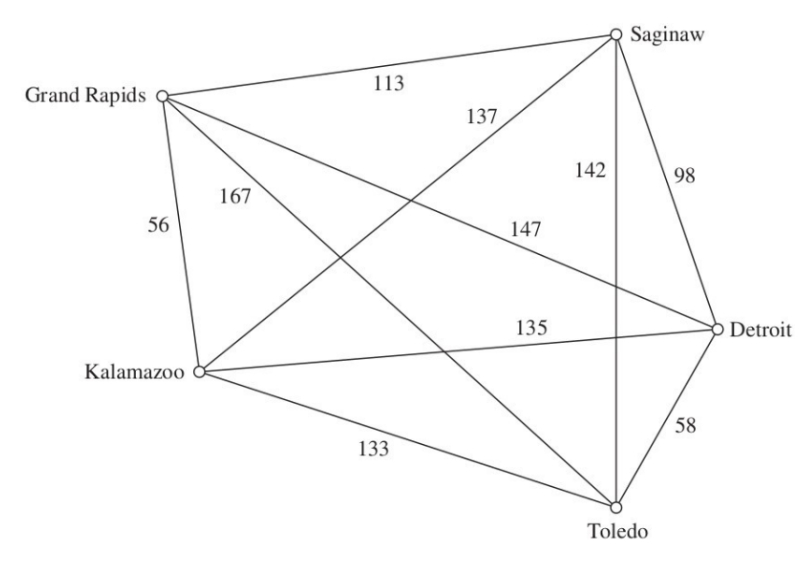
\includegraphics[width=0.75\textwidth]{C:/Users/Jhoel/Documents/python/homeworks/practica 3/Reporte/imagenes/figura1.png}
		\caption{Representación del problema del agente viajero utilizando un grafo.}
	\end{figure}
	\begin{itemize}
		\item La ruta más corta tiene una ongitud de 458.0.\\
		\item El ciclo Hamiltoniano más óptimo es el de Grand Rapids, Saginaw, Detroit, Toledo, Kalamazoo y Grand Rapids.
		\item El tiempo de ejecucion del algoritmo fue de 1.495 segundos.
	\end{itemize}
	\subsection{Incrementando el número de nodos aleatoriamente}
	Para la generación de las matrices de prueba se utilizó los siguientes parámetros:
	\begin{enumerate}
		\item Numero de nodos = [50, 100, 200, 1000]
		\item Rango de distancias = entre 50 a 150
	\end{enumerate}
	Se utilizaron los mismos parámetros para el algoritmo
	En la siguiente tabla se muestra la influencia que tiene el número de nodos (ciudades) frente al tiempo.
	
	\begin{table}[ht]
		\centering
		\begin{tabular}{cc}
			\hline
			Nro de Nodos & Tiempo (s)\\
			\hline
			50 & 19.33\\
			100 & 42.78\\
			200 & 100.98\\
			1000 & 1089.91\\
			\hline
		\end{tabular}
		\caption{Se muestra el incremento de nodos frente a los tiempos de ejecución obtenidos por el algoritmo}
	\end{table}
	
	A conticuación se muestra los graficos de distancia total vs el número de iteraciones de  cada número de nodos. El grafico muestra la evolucion del algoritmo, como poco a poco las hormigas artificiales buscan un camino más corto.\\
	\begin{figure}[H]
		\centering
		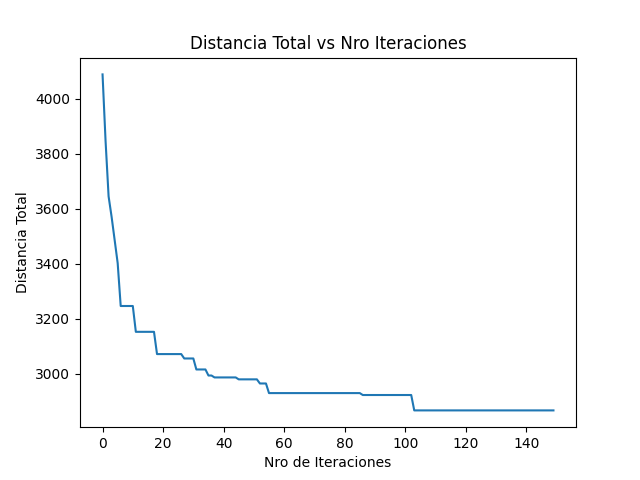
\includegraphics[width=0.75\textwidth]{C:/Users/Jhoel/Documents/python/homeworks/practica 3/Reporte/imagenes/Figure_2.png}
		\caption{Representación de las distancias totales vs el número de iteraciones de un TSP de 50 nodos}
	\end{figure}
	\begin{figure}[H]
		\centering
		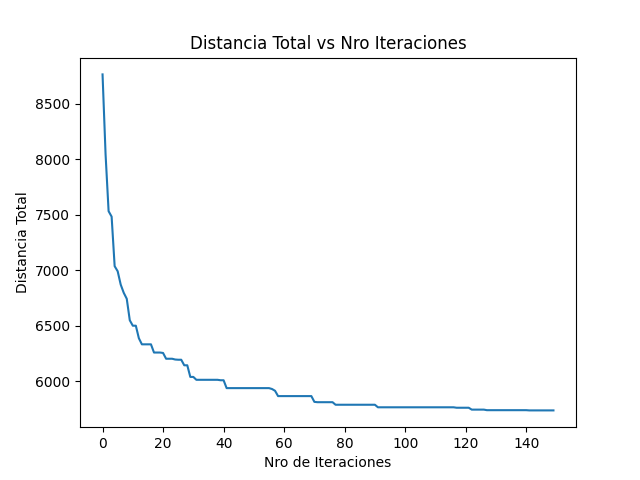
\includegraphics[width=0.75\textwidth]{C:/Users/Jhoel/Documents/python/homeworks/practica 3/Reporte/imagenes/Figure_3.png}
		\caption{Representación de las distancias totales vs el número de iteraciones de un TSP de 100 nodos}
	\end{figure}
	\begin{figure}[H]
		\centering
		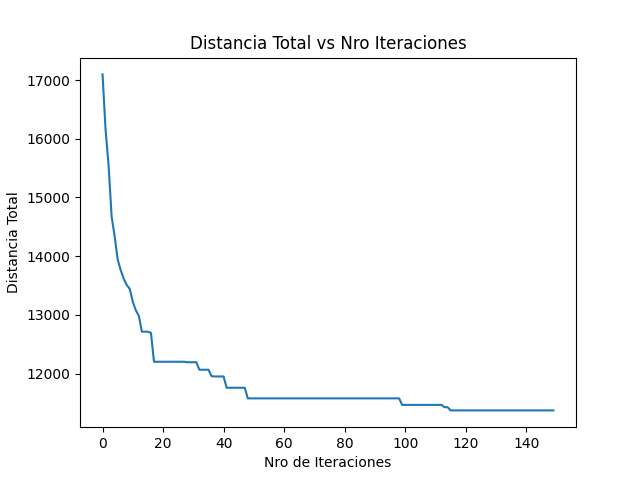
\includegraphics[width=0.75\textwidth]{C:/Users/Jhoel/Documents/python/homeworks/practica 3/Reporte/imagenes/Figure_4.png}
		\caption{Representación de las distancias totales vs el número de iteraciones de un TSP de 200 nodos}
	\end{figure}
	\begin{figure}[H]
		\centering
		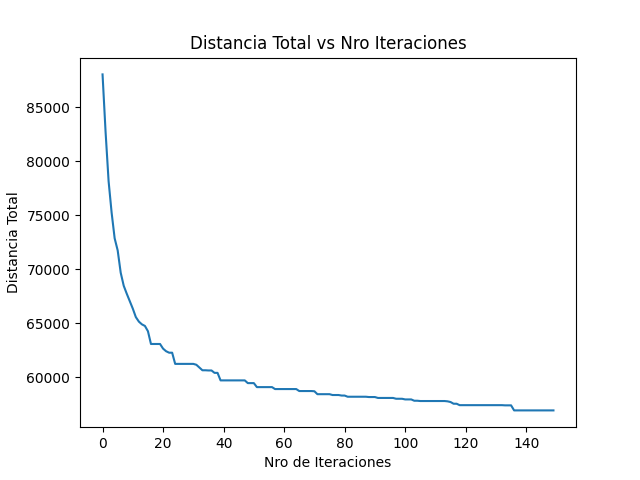
\includegraphics[width=0.75\textwidth]{C:/Users/Jhoel/Documents/python/homeworks/practica 3/Reporte/imagenes/Figure_5.png}
		\caption{Representación de las distancias totales vs el número de iteraciones de un TSP de 1000 nodos}
	\end{figure}
	
	\subsection{Variando el Número de hormigas}
	En el siguiente cuadro se muestra como varia el tiempo de ejecución a medida que el número de hormigas incrementa
	\begin{table}[ht]
		\centering
		\begin{tabular}{cccc}
			\hline
			Nro de Nodos & Número de Hormigas & Tiempo (s)& Distancia Total\\
			\hline
			50 & 50& 20.14&2900.0\\
			50 & 60& 24.05&2901.0\\
			50 & 70&27.63&2879.0\\
			50 & 80&31.45&2850.0\\
			50 & 90&35.43&2874.0\\
			50 & 100&39.68&2868.0\\
			50 & 110&44.69&2808.0\\
			50 & 120&45.97&2847.0\\
			50 & 130&49.83&2865.0\\
			50 & 140&53.54&2856.0\\
			\hline
		\end{tabular}
		\caption{Se muestra el tiempo de ejecución y la distancia frente a una misma matriz de distancias}
	\end{table}
	
	Se puede observar que al principio, la calidad de la respuesta mejora a medida que se incrementa la cantidad de hormigas.
	
	\section{Conclusiones}
	El algoritmo de Colonia de Hormigas es una herramiento poderosa y versatil para resolver el problema del agente viajero\\
	
	Este algoritmo depende en gran medida de los parámetros iniciales. Esto quiere decir que incrementar o decrementar la cantidad de hormigas, porcentaje de evaporación, alpha, beta y los demas parámetros afectan significativamente en el rendimiento del algoritmo.
	
\end{document}
